\documentclass[legalpaper, 12pt]{book}
\usepackage[utf8]{inputenc}
\usepackage[english]{babel}
\usepackage{amsmath}
\usepackage{amsfonts}
\usepackage{amssymb}
\usepackage{graphics}
\usepackage{xcolor}
\usepackage[pdftex]{hyperref}

\begin{document}

The exercise made here was based on the chapters of Panorama Technologies book (Chapter 2 Seismic Modeling) plus some personal adjustments.

The acoustic wave equation for a medium of constant density is defined by:

\[ \frac{\partial^2 U}{\partial t^2} = V^2 \nabla^2 U \]

Where $U$ and $V$ represents the pressure (or displacement) and velocity fields. For 1D case it gets simplified to:

\begin{equation}
\frac{\partial^2 U}{\partial t^2} = V^2 \frac{\partial^2 U}{\partial x^2}
\label{eq:wave1d}
\end{equation}

From equation (\ref{eq:wave1d}) we can approximate time derivatives by Taylor series, manipulating we can reach the following  central differences recursive formula:
\[ \frac{\partial^2 U}{\partial t^2} = \frac{1}{\Delta t^2} \left( U(t+\Delta t) -2 U(t) + U(t-\Delta t) - \sum_{i=2}^{i=\infty} \frac{\partial^{2i} U}{\partial t^{2i}} \frac{\Delta t^{2i}}{2i!} \right) \]

Where the first term is the second order approximation. For a fourth order approximation in time we use $i=2$ that gives:

\begin{equation}
\frac{\partial^2 U}{\partial t^2} = \frac{1}{\Delta t^2} \left( U(t+\Delta t) -2 U(t) + U(t-\Delta t) - \frac{\partial^{4} U}{\partial t^{4}} \frac{\Delta t^{4}}{12}\right)
\label{eq:partial4}
\end{equation}

Now we gonna use the wave equation to find $\frac{\partial^{4} U}{\partial t^{4}}$. If we differentiate equation (\ref{eq:wave1d}) twice in time we can have:

\begin{eqnarray}
\frac{\partial^4 U}{\partial t^4} &=& \frac{\partial^2 }{\partial t^2} \left( V^2 \left( \frac{\partial^2 U}{\partial x^2} \right) \right) \nonumber \\
& =&  V^2 \frac{\partial^2 }{\partial t^2} \frac{\partial^2 U}{\partial x^2} \nonumber \\
&=&  V^2 \frac{\partial^2 }{\partial x^2} \frac{\partial^2 U}{\partial t^2}  \mbox { since U is $C^2$ class function } \nonumber \\
&=& V^2 \left( \frac{\partial^2 V^2}{\partial x^2} \frac{\partial^2 U}{\partial x^2} + 2 \frac{\partial V^2}{\partial x} \frac{\partial^3 U}{\partial x^3} + V^2 \frac{\partial^4 U}{\partial x^4} \right) \nonumber \\
&=& V^2 \left\{ \left[ \left(  \frac{\partial V}{\partial x} \right)^2 + V  \frac{\partial^2 V}{\partial x^2} \right] 2 \frac{\partial^2 U}{\partial x^2} + 2 V \frac{\partial V}{\partial x}  \frac{\partial^3 U}{\partial x^3} +  V^2 \frac{\partial^4 U}{\partial x^4}\right\}
\label{eq:partial4final}
\end{eqnarray}

Finally merging (\ref{eq:partial4final}) with (\ref{eq:partial4}) we have an expression for the fourth order derivative in time. We used in this case  high order spatial derivatives from the spatial side of the original wave equation to make the "trick", helping to not use a huge stencil in time.

\begin{equation}
\frac{\partial^2 U}{\partial t^2} = \frac{U(t+\Delta t) -2 U(t) + U(t-\Delta t)}{\Delta t^2} - \frac{\Delta t^{2}}{12} V^2 \left\{ \left[ \left(  \frac{\partial V}{\partial x} \right)^2 + V  \frac{\partial^2 V}{\partial x^2} \right] 2 \frac{\partial^2 U}{\partial x^2} + 2 V \frac{\partial V}{\partial x}  \frac{\partial^3 U}{\partial x^3} +  V^2 \frac{\partial^4 U}{\partial x^4}\right\}
\end{equation}

For simplicity we will call the left side after the minus signal $LW$, then:

\begin{equation}
LW = \frac{\Delta t^{2}}{12} V^2 \left\{ \left[ \left(  \frac{\partial V}{\partial x} \right)^2 + V  \frac{\partial^2 V}{\partial x^2} \right] 2 \frac{\partial^2 U}{\partial x^2} + 2 V \frac{\partial V}{\partial x}  \frac{\partial^3 U}{\partial x^3} +  V^2 \frac{\partial^4 U}{\partial x^4}\right\} \\
\frac{\partial^2 U}{\partial t^2} = \frac{U(t+\Delta t) -2 U(t) + U(t-\Delta t)}{\Delta t^2} - LW
\label{eq:partialEnd}
\end{equation}

From here we can write a explicit forward matching algorithm for data synthesis for the wave equation. Those methods are also known as quadrature methods.  So going back to the wave equation (\ref{eq:wave1d}) we can use fourth order for the spatial derivatives (central differences) together with fourth order time derivative that we found (\ref{eq:partialEnd}). Doing that we get:

\begin{equation}
\frac{\partial^2 U}{\partial t^2} = \frac{{V_j^n}^2}{\Delta x^2} \sum_{i=-2}^{2} w_i^b U_{j+i}^n  \\
\frac{U_j^{n+1} -2 U_j^n + U_j^{n-1}}{\Delta t^2} -LW_j^n = \frac{{V_j^n}^2}{\Delta x^2} \sum_{i=-2}^{2} w_i^b U_{j+i}^n \\
U_j^{n+1} = \Delta t^2 \left( \frac{{V_j^n}^2}{\Delta x^2} \sum_{i=-2}^{2} w_i^b U_{j+i}^n +LW_j^n \right) +2 U_j^n - U_j^{n-1}
\end{equation}

and the $LW$ term will be:

\begin{equation}
LW_j^n = \frac{\Delta t^{2}}{12 \Delta x^4} {V_j^n}^2 \left\{ \left[ \left( \sum_{i=-2}^{2} w_i^a V_{j+i}^n \right)^2 + V_j^n \sum_{i=-2}^{2} w_i^b V_{j+i}^n  \right] 2 \sum_{i=-2}^{2} w_i^b U_{j+i}^n + 2 V_j^n \sum_{i=-2}^{2} w_i^a V_{j+i}^n \sum_{i=-3}^{3} w_i^c U_{j+i}^n +  {V_j^n}^2 \sum_{i=-3}^{3} w_i^d U_{j+i}^n \right\}
\end{equation}

Where the coefficients are given by:

\[ w^a = \frac{1}{12} [1, -8, 0, 8, -1] \mbox { first derivative } \]
\[ w^b = \frac{1}{12} [-1, 16, -30, 16, -1]  \mbox { second derivative }\]
\[ w^c = \frac{1}{8} [1, -8, 13, 0, -13, 8, -1]  \mbox { third derivative }\]
\[ w^d = \frac{1}{6} [-1, 12, -39, 56, -39, 12, -1 ] \mbox { fourth derivative }\]

We used $ j $ as index of discretization in space and $ n $ for time. The coefficients $ w $ for the central derivatives were obtained from the table bellow, from \hyperlink{wiki}{\hypertarget{http://en.wikipedia.org/wiki/Finite_difference_coefficients}}

\begin{figure}
\centering
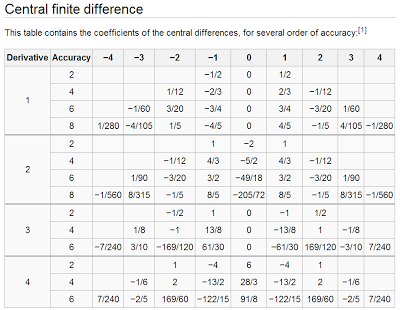
\includegraphics[width=0.7\linewidth]{./Central finite difference coefficients}
\caption{}
\label{fig:Centralfinitedifferencecoefficients}
\end{figure}
\newpage
\end{document}